\documentclass[12pt,a4paper]{article}
\usepackage[utf8]{inputenc}
\usepackage{amsmath}
\usepackage{amsfonts}
\usepackage{amssymb}
\usepackage[margin = 1in, bottom=1in, top=1in]{geometry}
\usepackage{fancyhdr}
\usepackage{graphicx}
\usepackage{titlesec}
\usepackage{float}
\usepackage{amsmath}
\usepackage[utf8]{inputenc}
\usepackage[english]{babel}
\usepackage{siunitx}
\usepackage{hyperref}
\usepackage[all]{hypcap}
\usepackage[export]{adjustbox}
\usepackage{textcomp}
\usepackage{gensymb}
\usepackage{physics}
\usepackage[nottoc,notlot,notlof]{tocbibind}
\newcommand\tab[1][1cm]{\hspace*{#1}}
\parindent 0ex
\titleformat{\subparagraph}
    {\normalfont\normalsize\bfseries}{\thesubparagraph}{1em}{}
\titlespacing*{\subparagraph}{\parindent}{3.25ex plus 1ex minus .2ex}{.75ex plus .1ex}
\usepackage[acronym,nomain]{glossaries}
\usepackage{slashbox}
\usepackage[acronym]{glossaries}




\titleformat{\paragraph}
{\normalfont\normalsize\bfseries}{\theparagraph}{1em}{}
\titlespacing*{\paragraph}
{0pt}{3.25ex plus 1ex minus .2ex}{1.5ex plus .2ex}
\setcounter{secnumdepth}{4}
\setcounter{tocdepth}{4}

\renewcommand{\headrulewidth}{0pt}


\fancypagestyle{a}{\fancyhf[L]{
\includegraphics{1.jpg}}\fancyhead[R]{
\includegraphics[scale=0.25]{2.jpg}}\fancyfoot[]}

\begin{document}

\begin{titlepage}
\begin{center}
\setcounter{page}{1}

\thispagestyle{a}
\vspace*{2cm}
\huge{\textbf{CIRCUIT DESIGN PROJECT WS 17/18}} \\[4mm]
\Large{\textbf{Hochschule Ravensburg - Weingarten}}\\ [1.5cm]

\line(1,0){450}\\
Measurement of the time per rotation of the Turning Table \\
\line(1,0){450}\\ [0.75cm]




\begin{tabbing}
\hspace{6cm}\=\hspace{4.5cm}\=\kill
 Project By: \> Mehul Amipara (25809)   \>  \\
  \> Prithvi Patel (27890) \>   \\ \\
 Guided By: \>Dr.-Ing., Professor Walter Ludescher  \>    \\ 
  \> Dipl.-Ing.(FH), Christoph Weber\>  \\ \\
 
   Submitted on:   \> 24.01.2018 \> 
\end{tabbing} 


\end{center}
\end{titlepage}

\newpage
\pagestyle{fancy}
\fancyfoot{}
\fancyhead{}

\setlength{\footskip=0pt}
\setlength{\headheight=35pt}

\newpage


\section*{Acknowledgement}

We are glad to express our indebtedness to our guide Prof. Dr. Walter Ludescher, Department of Electrical Engineering and Information Technology, Hochschule Ravensburg - Weingarten, for his valuable time and guidance, constant encouragement and kind help at various stages for the execution of the project task.\\

We are also thankful to Mr. Weber, Department of Electrical Engineering and Information Technology, for providing valuable assistance and insight during the experimental process.\\

Also, Many students, especially my classmates and team member himself, have made valuable suggestions on this proposal which gave us an inspiration to improve our assignment. We are thankful to all the Students who help me in order to improve and execute our Assignment.\\

\newpage
\section*{Abstract}
In this Project, We have designed a Circuitry by using VHDL(Very High Speed Integrated Circuit Hardware Description Language) Programming Language.  This Project leads to the result of the Measurement of the time per rotation taken by the disk on the Turning Table. So, How it works! Here it goes : First of all, the Sensor that has been used for the Hardware Setup is an Infrared Sensor. The Circuitry gets a pulse, a Raw Sensor Signal, from the Sensor when a piece of block placed on the disk cuts the infrared line of the sensor. The neat or clear Sensor signal is required in order to use it for the counter. The cleaning part has been carried out by one of the blocks in between. The counter calculate the time taken by the disk for a single rotation and has been sent to the host computer by using UART and RS-232 protocol. The Project involves the Circuit designing using VHDL, a Hardware Description Language. Testing of the VHDL code has been done on the Spartan 3E Board. We have designed our Circuitry to make the calculations as accurate as possible. We had put our hard efforts to make it accurate so that for the large scale production of the chips executing this circuitry can be an optimal design.\\


\newpage
\section*{Requirement and Objectives of the project}
The objective of this project is to learn how an engineer should design the Circuitry using VHDL programming, how things actually works in the real world. The ultimate target is to find the time of a single rotation taken by the disk on the Turning Table. The FPGA development board that has been used for this project is Spartan 3E FPGA development Board. The VHDL code that has been developed during this project is designed to take the pulse that comes from the sensor and when it detects that pulse, it start counting and increments the counter at every one millisecond. After some milliseconds, around 2000 counts ideal but it depends on the speed of the disk rotating, when it detects the second pulse that’s coming from the sensor, then the counter stops counting and then is been sent to the computer via UART considering RS-232 protocol. Then there exist a C source code that reads the data that’s coming from the port where the output of the FPGA board is connecting, it reads the values and print it on the command line terminal. For testing, GTKterm has been used for the project.\\

There were certain requirement that has also been taken into consideration:
\begin{itemize}
\item The requirement is that the time that has been counted by the counter and then after sent to the transmission block, it should send the data at the Baud rate 9K6 Hz or 9600 Hz.\

\item Finite State Machine algorithm has been used to prevent latches.

\item The whole block should have at least 4 signals: reset, clock, sensor signal, and txd signal.\

\item Clock speed is required to be 50MHz, but in this design, one more specialty is added, that is, this system can be completely synchronised for 50MHz as well as 10 MHz. There is a switch in between when the design gives results in 50Mhz as well as 10Mhz with using just a switch.\

\item The transmission should be using UART considering RS-232 protocol.\
\end{itemize}

In the top level, it seems like that there is just a single block that has been doing all the work. But actually, it works quite opposite. It has been divided into multiple small blocks that carries out small tasks and at the end, when all the blocks are connected, it seems like something big is happening. 




\newpage
\pagestyle{fancy}
\fancyfoot{}
\fancyhead{}
\setlength{\footskip=25pt}
\setlength{\headheight=0pt}
%\renewcommand{\footrulewidth}{0.4pt}

\fancyfoot{}
\newpage

\rfoot{Page $\vert$ \thepage}
\pagenumbering{roman}
\setcounter{page}{5}
\tableofcontents
\clearpage

\section*{Section with acronyms}



\newacronym{gcd}{GCD}{Greatest Common Divisor}
\newacronym{lcm}{LCM}{Least Common Multiple}
\printglossary[type=\acronymtype]


\addcontentsline{toc}{section}{\listfigurename}
\listoffigures
\clearpage


\fancyfoot{}
\rfoot{\thepage}
\pagenumbering{arabic}
\setcounter{page}{1}
\renewcommand{\baselinestretch}{1.5} % line space
\section{Introduction}
There are certain arrangements needed in order to do the design of this Circuitry, such as the Hardware Setup, Software Setup for Stimulation and Software to upload the code to the FPGA board. These things are going to be discussed in this Chapter. In order to upload the code into the FPGA board, a short description is required for the FPGA.\

%\thispagestyle{c}
\subsection{Introduction to FPGA }
A Field Programmable Gate Array (FPGA) is a semiconductor device containing programmable logic components and programmable interconnects. The programmable logic components can be programmed to duplicate the functionality of basic logic gates such as AND, OR, NOT, XOR or more complex combinational functions such as decoders or math functions. The FPGA configuration is generally specified using a hardware description language (HDL). The most common FPGA architecture consists of an array of logic blocks called Configurable Logic Block (CLB) or Logic Array Block (LAB), I/O pads- to make off chip connections and programmable routing channels to implement logical functions. FPGAs have analogue features in addition to digital functions. The most common analogue feature is programmable slew rate and drive strength on each output pin. Another relatively common analogue feature is differential comparators on input pins designed to be connected to differential signalling channels.\\

\begin{figure}[H]
\centering
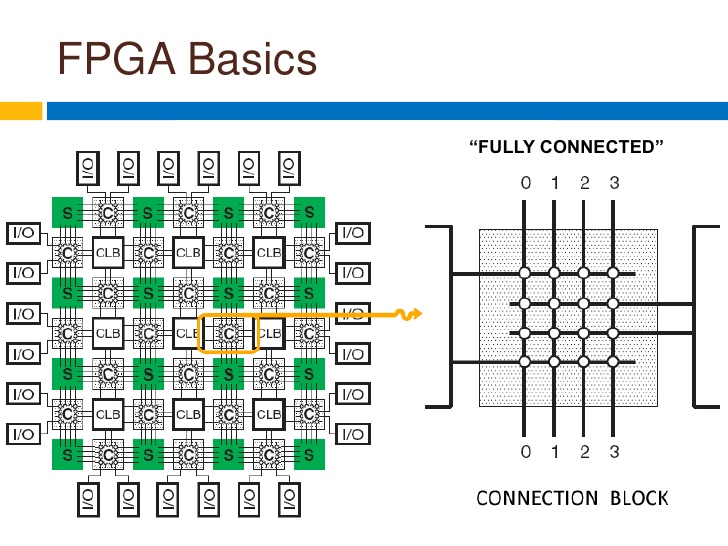
\includegraphics[height=10cm,width=11.5cm]{FPGA.jpg}
\caption{General Architecture of FPGA}
\label{General Architecture of FPGA}
\end{figure}

\subsection{Introduction to the hardware used for the Project}
The Spartan 3E FPGA development Board provides all the basic features and said to logically optimized.
\begin{itemize}

\item For applications where logic densities matters more than I/O count.\
\item Ideal for logic integration, DSP co-processing and embedded control, requiring significant processing and narrow or few interfaces.
\end{itemize}

For the project, Spartan 3E: XC3S500E: FG320 has been used.\ 

\begin{figure}[H]
\centering
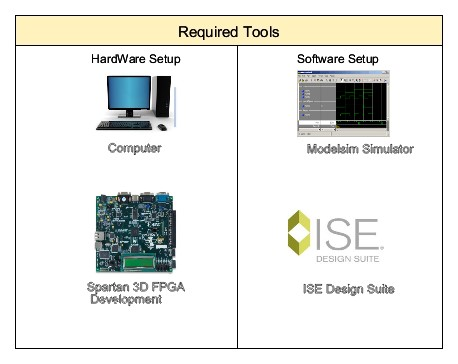
\includegraphics[width=11.5cm,height=9cm]{Required.jpg}
\caption{General Architecture of FPGA}
\label{Required.jpg}
\end{figure}

The Spartan 3E FPGA board comes built in with many peripherals that help in the proper working of the board and also in interfacing the various signals to the board itself. Some of the peripherals are:\

\begin{itemize}
\item 2-line, 16 Character LCD screen \
\item PS/2mouse/keyboard port \
\item VGA display port\
\item Two 9-pin RS-232 ports\
\item 50 MHz clock oscillator\
\item On-board USB-based FPGA download and debug interface\
\item Four slide switches and four push-button switches\

\end{itemize}

Moreover, The Spartan-3 family architecture consists of five fundamental programmable functional elements: Configurable Logic Blocks (CLBs) contain RAM-based Look Up Tables (LUTs) to implement logic and storage .Elements that can be used as flip-flops or latches. CLBs can be programmed to perform a wide variety of logical functions as well as to store data. Input/output Blocks (IOBs) control the flow of data between the I/O pins and the internal logic of the device. Each IOB supports bidirectional data flow plus 3-state operation. Twenty-six different signal standards, including eight high performance differential standards, are available. Block RAM provides data storage in the form of 18-Kbit dual-port blocks. Multiplier blocks accept two 18-bit binary numbers as inputs and calculate the product. Digital Clock Manager (DCM) blocks provide self-calibrating, fully digital solutions for distributing, delaying, multiplying, dividing, and phase shifting clock signals.\\

\subsection{Information about VHDL}
VHDL(VHSIC-Very High Speed Integrated Circuit  Hardware Description Language)  is a hardware description language used in electronic design automation to describe digital and mixed-signal systems such as field-programmable gate arrays and integrated circuits. VHDL can also be used as a general purpose parallel programming language.
VHDL is commonly used to write text models that describe a logic circuit. Such a model is processed by a synthesis program, only if it is part of the logic design. A simulation program is used to test the logic design using simulation models to represent the logic circuits that interface to the design. This collection of simulation models is commonly called a testbench.\\
A VHDL simulator is typically an event-driven simulator. This means that each transaction is added to an event queue for a specific scheduled time. E.g. if a signal assignment should occur after 1 nanosecond, the event is added to the queue for time +1ns. Zero delay is also allowed, but still needs to be scheduled: for these cases Delta delay is used, which represent an infinitely small time step. The simulation alters between two modes: statement execution, where triggered statements are evaluated, and event processing, where events in the queue are processed.\\
VHDL has constructs to handle the parallelism inherent in hardware designs, but these constructs (processes) differ in syntax from the parallel constructs in Ada (tasks). Like Ada, VHDL is strongly typed and is not case sensitive. In order to directly represent operations which are common in hardware, there are many features of VHDL which are not found in Ada, such as an extended set of Boolean operators including NAND and NOR.\\
VHDL has file input and output capabilities, and can be used as a general-purpose language for text processing, but files are more commonly used by a simulation testbench for stimulus or verification data. There are some VHDL compilers which build executable binaries. In this case, it might be possible to use VHDL to write a testbench to verify the functionality of the design using files on the host computer to define stimuli, to interact with the user, and to compare results with those expected. However, most designers leave this job to the simulator.\\
It is relatively easy for an inexperienced developer to produce code that simulates successfully but that cannot be synthesized into a real device, or is too large to be practical. One particular pitfall is the accidental production of transparent latches rather than D-type flip-flops as storage elements.\\
One can design hardware in a VHDL IDE (for FPGA implementation such as Xilinx ISE, Altera Quartus, Synopsys Synplify or Mentor Graphics HDL Designer) to produce the RTL schematic of the desired circuit. After that, the generated schematic can be verified using simulation software which shows the waveforms of inputs and outputs of the circuit after generating the appropriate testbench. To generate an appropriate testbench for a particular circuit or VHDL code, the inputs have to be defined correctly. For example, for clock input, a loop process or an iterative statement is required$[12]$\\
A final point is that when a VHDL model is translated into the "gates and wires" that are mapped onto a programmable logic device such as a CPLD or FPGA, and then it is the actual hardware being configured, rather than the VHDL code being "executed" as if on some form of a processor chip.\\



\newpage

\renewcommand{\baselinestretch}{1.5} % line space
\section{GUIDELINES AND REQUIREMENT}
Everything related to circuit designing with VHDL will be discussed in this Chapter. This chapter includes the design guidelines that has to be done while programming with VHDL. These guidelines are ideal and are currently used worldwide. This chapter also describes the requirements that need to be fulfilled.\\

\subsection{Design Guidelines}
There are certain guidelines that need to follow:\\

\begin{enumerate}


\item A filename or dirname MUST NOT start with a special char or a number. \
\item A dot MUST BE used as a separator between filename and its extension.\\
	Example :     \hspace{1cm} content of the file has to be\\
	mycirc\_e.vhd \hspace{1cm} a VHDL-entity called mycirc\_e\\
	mycirc\_a.vhd \hspace{1cm} a VHDL-entity called mycirc\_a or mycirc\_a1\\
	README.txt    \hspace{1cm} some text\\

\item VHDL directories should be in the Tree Structure. This tree structures of four more directories inside(Documentation, Presentation, gcc and VHDL). The documentation directory consists of a report.pdf file(file name can be anything). The Presentation directory should consist a presentation.ppt or .pptx (filename can be anything). The gcc directory consists of the C-code that reads the data coming from the port ttyS0. The VHDL code should have the three more directories, sim – it consists of the simulation work file used in ModelSim to stimulating the code; src – it consists of the all the files related to VHDL program with the top level file.\

\item In source files, Each ENTITY has its own file. Each ARCHITECTURE has its own file. And each Architecture has its own TESTBENCH(es).\
\item Use of TABS is forbidden.\
\item Using more than 80 characters per line is forbidden.\ 
\item For signal-names in entities, the following rule should be applied:\
\begin{itemize}
\item rb\_i \hspace{1cm} 	: input, async. Global reset, active low\
\item cp\_i \hspace{1cm}  	: input, async. Global System clock, active at rising edge \
\item xx\_i \hspace{1cm}  	: input signal named xx\_i\
\item xx\_o \hspace{1cm}    : output signal named xx\_o\
\item xy\_io\hspace{1cm} 	: in-out signal\
\end{itemize}

\item For all signals in Architecture, rules are : xyz\_s  : an internal signal named xyz\_s\
\item All architectures containing memory must have an input called rb\_i and cp\_i.\
\item All architecture containing no memory must not have an input called rb\_i  and cp\_i.\
\item Constants and components must be defined in a Package\


\end{enumerate}


\subsection{Requirements}
There are certain requirements that need to be fulfilled. This requirement section basically consists of Hardware requirements and software requirements.\\

The Hardware requirements includes :\
\begin{itemize}
\item A turning table set up for calculating the speed of a single rotation of the Disc.\
\item An infrared sensors placed on the turning table\
\item DB9 RS-232 Cable from FPGA board to PC\
\item System Clock and Asynchronous Reset button\
\item A DILIGANT Spartan 3E FPGA board for circuit implementation(for counting and measurement)\
\item UART for data transmission to PC\
\item PC with UART interface\
\end{itemize}

The Software requirements includes :\
\begin{itemize}
\item VHDL for Programming FPGA and UART\
\item C-code for printing the data coming from the port ttyS0 at the baudrate 9600 Hz\
\item MODELSIM or System Simulation\
\item ISE for synthesizing the VHDL program and uploading to the FGPA board\
\end{itemize}

\newpage

\renewcommand{\baselinestretch}{1.5} % line space
\section{CIRCUIT DESIGNING WITH VHDL}
A brief overview of the top level of the Circuit blocks will be described in this chapter. Moreover, the top level consists of some small blocks such as counters, multiplexers,etc is going to described in this chapter.\\


\subsection{Top Level Block Diagram Entity}

\begin{figure}[H]
\centering
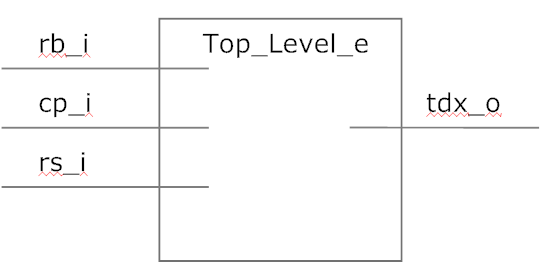
\includegraphics[width=8cm,height=6cm]{TopLevelE.PNG}
\caption{Top Level Entity}
\label{Top Level Entity}
\end{figure}


\begin{enumerate}
\item \textbf{cp\_i:} cp\_i denotes the system clock. It is a contineous sequence of low and High on the line providing to it. The system clock is needed to synchronize all the components that is running on the FPGA board. That means, they all do their work only if the clock is high;never when it’s low. And because of the clock speed is set above the longest time any signal needs to propogatethrough any circuit on the board,this signals is preventing signals from arriving before other signals and thus makes everything safe and synchronyzed.

\item \textbf{rb\_i:} rb\_i denotes the reset button signal. It is an active low signal. It is a signal that initialize the complete system. Reset can be switch button or a push button and is generally used by the user. It restart all the interfaces and all the State Machines which are working inside the FPGA chip, are forced to go to its initial state. 

\item \textbf{rs\_i:} rs\_i is the signal that is coming from the sensor, that is placed on the Turning table setup. The sensor that is used for the project is a infrared sensor and it detects the disturbance that comes inbetween its infrared line. With the help of this signal, the system starts counting.

\item \textbf{txd\_o:} txd\_o is the signal that send a serial line of data that is processed inside the system. That means, the data that comes are the bits that are sent in UART sequence corresponding to the RS-232 Protocol. In this project, the conversion of the counter value that is counted by BCD counter is done in to the ASCII vector and this vector is then transmitted via txd\_o signal in a particular sequence. This sequence will be described later.

\item There were also some other signals that has been taken out, just for testing purpose.
\end{enumerate}

Here, the signals from the top\_level entity have been discussed. The Architecture is declared and explained in the next Section.\

\begin{figure}[H]
\centering
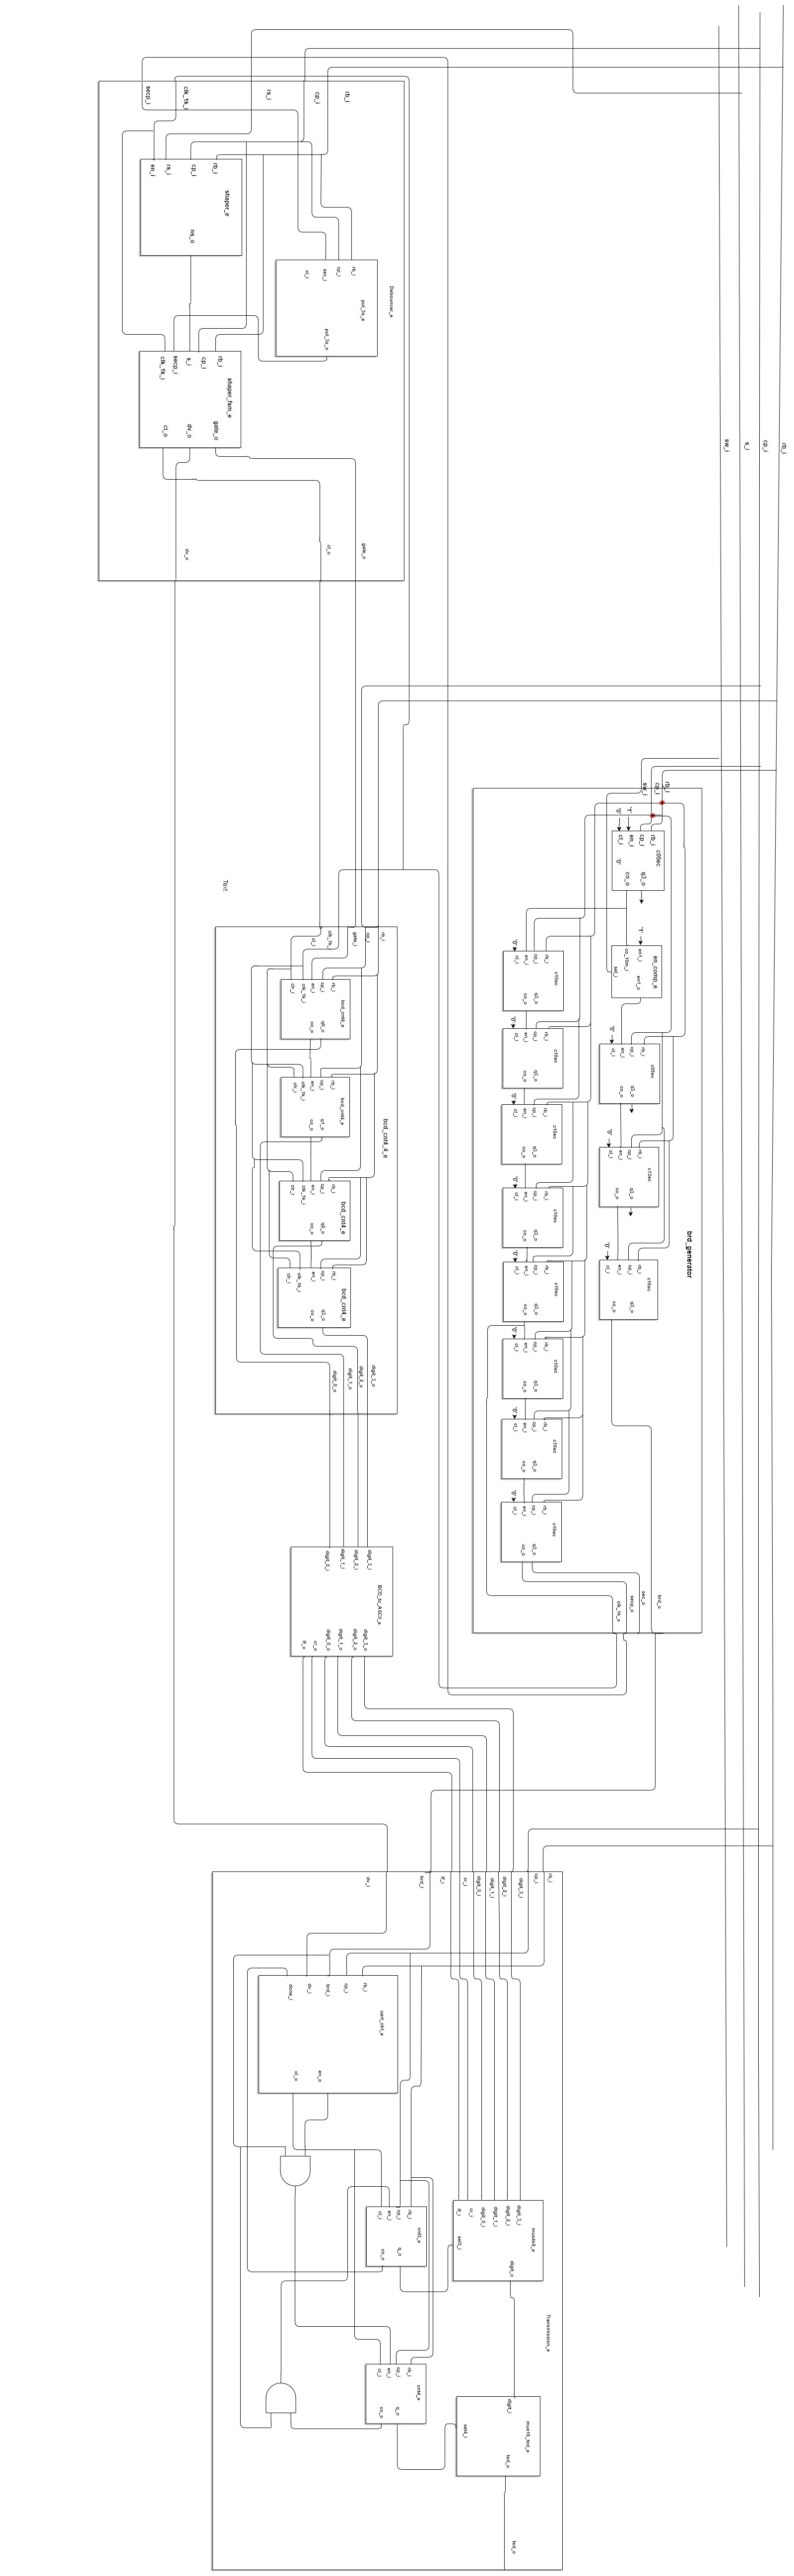
\includegraphics[width=16cm,height=23cm]{Toplevel.jpg}
\caption{Top Level Architecture}
\label{Top Level Architecture}
\end{figure}
\newpage



\subsection{Top level block diagram Architecture}
As it can be seen, the top level architecture is a very big schematic and it is very hard to understand everything at a single glance. Basically, it provides an algorithm that calculates the speed of the disk rotating at a particular speed. It gives the output in milliseconds. That’s the accuracy it provides. \

As it becomes a bit complicated to understand, let’s try to break it down into small modules. The very first module through which the sensor signal passes, is the Debouncer. Debouncer is basically a block in the top level architecture that debounce the incoming sensor signal. That means, it is very important block in the system architecture and is responsible for starting and stopping the value of the timing taken per rotation in correspondence to the sensor signal. It is also responsible for activating the UART(transmission block).\
 
The next module is the brd\_generator. It is also a very important block and consists of the running counters and it gives output as dividing frequency of 9600 Hz. This divided frequency is used as a baud rate for transmitting the data. There is one more frequency divided signal called as the clk\_1k signal which is used for process the sensor signal and for calculating the time taken between two sensor signals.\

The next module is the BCD\_counter. It is a counter that counts the value upto 4 digits. It is synchronized with the 1 millisecond pulse that is coming from the brd\_generator.  With the help of this clk\_1k signal, it calculates the time taken between two sensor signals.\

The next block is BCD\_to\_ASCII converter. It basically converts the values that has been counted by the BCD Counter and converts it into the ASCII values, e.g., for the value $1 => 31$ $||$ $0001 => 00110001$. This ASCII conversion is done by this block.

The last remaining and the most important module is the Transmission (UART) block. It is responsible for sending the ASCII data that is coming from the BCD\_to\_ASCII converter serially through a single signal. That is the output of the top level architecture and is connected to the computer.
\begin{figure}[H]
\centering
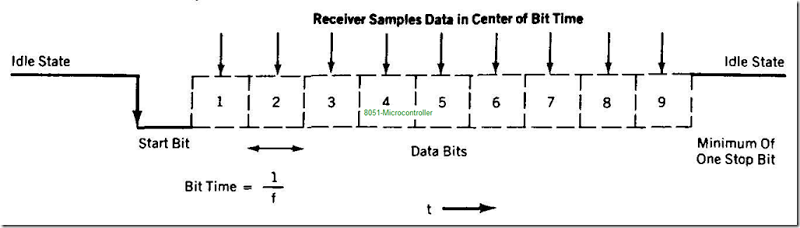
\includegraphics[width=\linewidth]{urattime.png}
\caption{The UART bit sequence }
\label{the UART bit sequence }
\end{figure}

So far, the overview of the top level architecture is explained. The detailed description of each block is given in the following sections.\

\subsection{Debouncer}
The entity of the Debouncer looks like :\\

\begin{figure}[H]
\centering
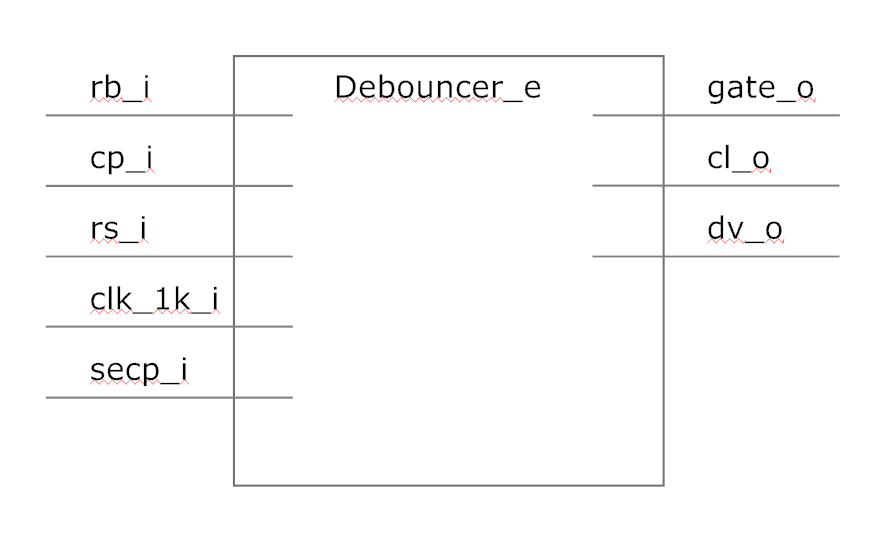
\includegraphics[width=8cm,height=6cm]{debouncere.PNG}
\caption{Debouncer Entity}
\label{Debouncer Entity}
\end{figure}

As mentioned above, this block is responsible for starting and stopping the values that is being counted by the BCD counter. The Debouncer module consists of three sub-blocks that fulfils all the functionality. The Debouncer is just a big block that consists of this three blocks namely shaper, shape\_fsm and pulse\_3s. The architecture of the debouncer looks like:

\begin{figure}[H]
\centering
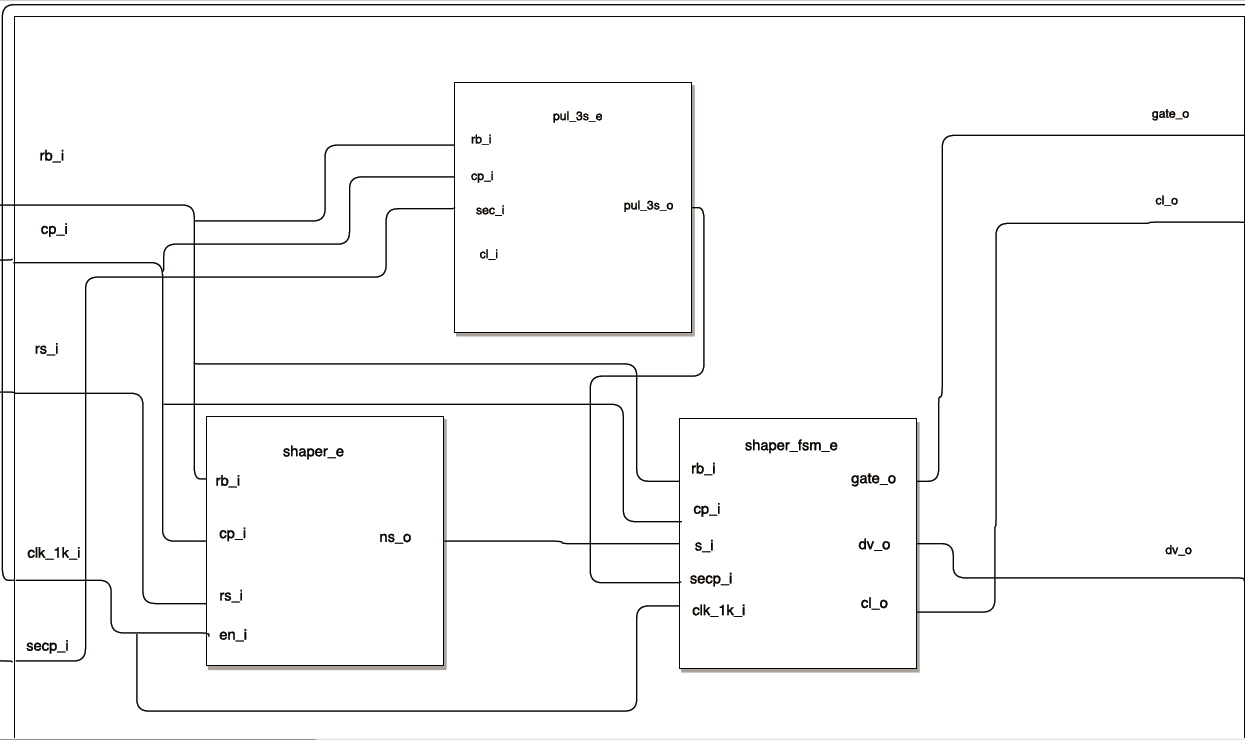
\includegraphics[width=16cm,height=10cm]{Debouncer_arc.PNG}
\caption{The architecture of the debouncer}
\label{the architecture of the debouncer}
\end{figure}

\begin{enumerate}
\item \textbf{Shaper :} Shaper is a block that filters the rough sensor signal that is coming from the sensor signal, from the infrared sensor. It basically consists of a counter that has 17 states and state transition occurs when the sensor signal is HIGH or ‘$1$’ and the EVENT of the clk\_1k(1 millisecond pulse) that is coming from the brd\_generator. When it appears that the current state is the 17th state and meanwhile if the raw sensor signal is HIGH or ‘1’ then it gives a pulse of 20 ns (system clock period) as an output signal. This process ultimately filters the sensor signal.

\begin{figure}[H]
\centering
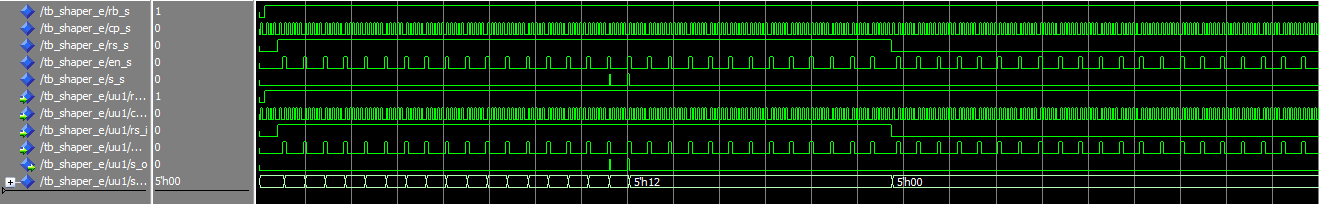
\includegraphics[width=15cm,height=5cm ]{shaper.PNG}
\caption{The timing behaviour of the shaper}
\label{the timing behaviour of the shaper}
\end{figure}

\item \textbf{Shaper\_fsm:} Shaper\_fsm is a block that activates the bcd\_counter module and Transmission(UART) block. The entity of the Shaper\_fsm has three outputs: gate signal, cl signal and dv signal. The gate signal is responsible for enabling the BCD counter. Unless and until this signal is HIGH or ‘$1$’, till then the BCD counter counts. The cl signal is responsible for clearing the bcd counters once the values’ been calculated and driven through the txd signal(output of the top level). The dv signal is responsible for enabling the transmission (UART) module.\


The working of the finite state machine goes here:\

\begin{figure}[H]
\centering
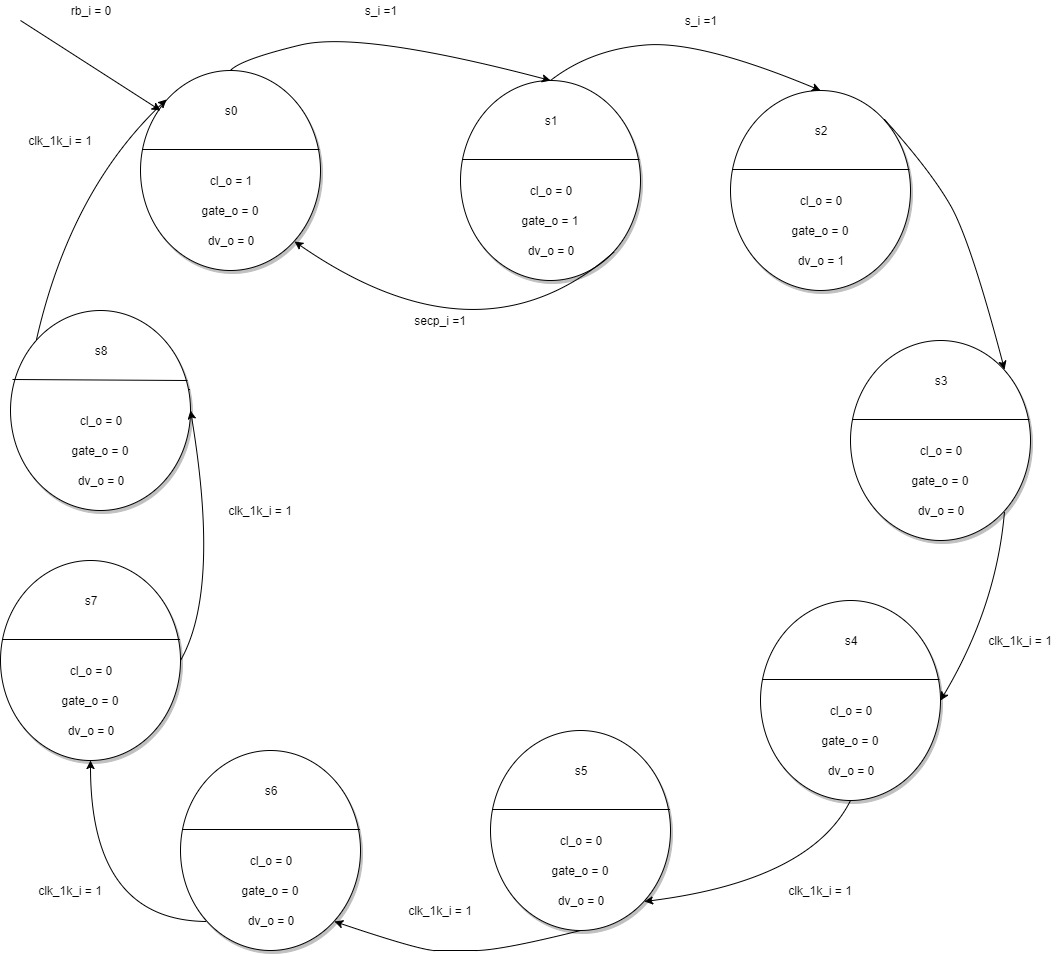
\includegraphics[width=10cm,height=8cm]{shaper_fsm.jpg}
\caption{Flow chart of the shaper fsm}
\label{Flow chart of the shaper fsm}
\end{figure}

At first, when the sensor detects the interruption, it gives a signal. This signal is roughly about 30 ms. When it detects the first sensor the signal, the gate signal goes to ‘$1$’. At this moment, the BCD counter starts counting. When the second sensor signal appears, the gate signal goes to ‘0’ and the dv signal goes to ‘$1$’.There is no condition needed for the state transition. The reason is that the pulse of 20 ns is enough to activate the Transmission (UART) module. Then, some delay has been given. This delay is of 6 ms and is exists there because if it goes to ‘$0$’ and the transmission has not been done, then it might give some weird or no required result. \
\[12\times 4\times 104000 ns= 4992000 ns => 5 ms \] 

This is the reason the delay of 6 ms have been chosen. Then after this delay, the cl signal goes to  ‘$1$’, that makes the BCD counter go to its initial state.\

\item \textbf{Pulse\_3s :}Pulse\_3e block gives a pulse every three seconds as soon as the sensor signal is detected. This works as a timeout counter that counts upto 3 seconds and if it still does not detect the second sensor pulse, then it just shut down the system and waits for the sensor pulse to start the counting.

\end{enumerate}

\subsection{Baud Rate Generator(brd\_generator)}
The Baud Rate Generator is basically composed of the counters. The calculations are something like :\

\[\frac{50 MHz}{5\times 5\times 13\times 16}= 9615.384Hz \Rightarrow 9600Hz \]

So, the design also looks similar to it. Moreover, This system is designed in such a way that it can run on the clock speed of 50 MHz as well as 10 MHz. There exists a switch, of which means the switching between two system clocks is possible.\
An Entity of the Baud Rate generator looks like:\\

\begin{figure}[H]
\centering
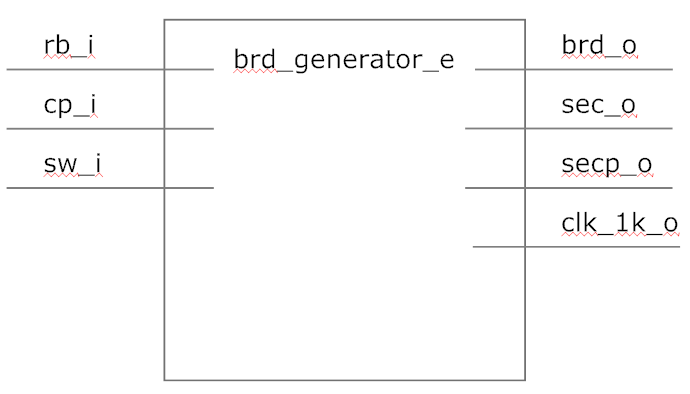
\includegraphics[width=8cm,height=7cm]{brdgeneratore.PNG}
\caption{ An Entity of the Baud Rate Generator}
\label{An Entity of the Baud Rate Generator}
\end{figure}

An architecture of the Baud Rate Generator looks like :\\
\begin{figure}[H]
\centering
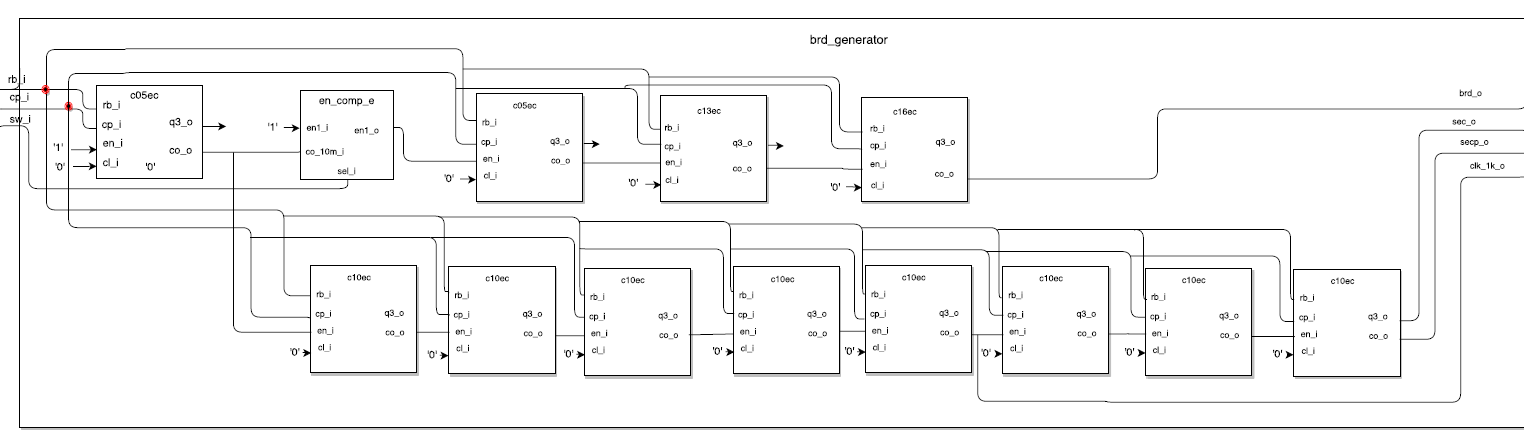
\includegraphics[width=16cm,height=7cm]{badGeneratorArc.PNG}
\caption{architecture of the Baud Rate Generator}
\label{architecture of the Baud Rate Generator}
\end{figure}

The timing behaviour of the brd\_generator looks like :\\
\begin{figure}[H]
\centering
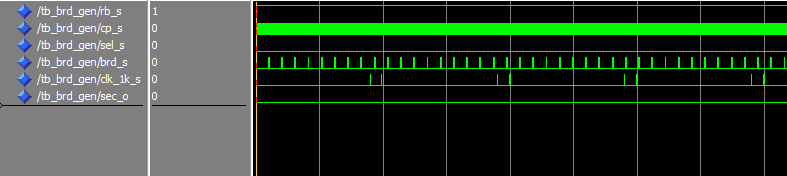
\includegraphics[width=16cm,height=5cm]{BaudRate.PNG}
\caption{The timing behaviour of the baud rate generator}
\label{the timing behaviour of the brd Generator}
\end{figure}

\subsection{BCD counter}
The BCD counter is responsible for counting the timing taken between two sensor signal pulses. This starts counting when the gate signal from the debouncer goes to ‘$1$’ and at every clk\_1k signal, it counts. \\

This is how the architecture of the BCD counter looks like :\\
\begin{figure}[H]
\centering
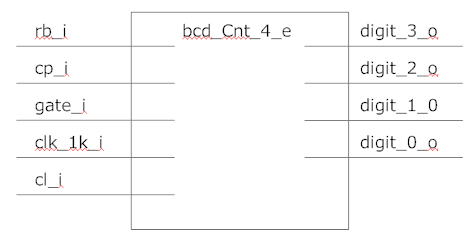
\includegraphics[width=8cm,height=6cm]{bcdCntE.PNG}
\caption{Entity of the BCD counter}
\label{Entity of the BCD counter}
\end{figure}

\begin{figure}[H]
\centering
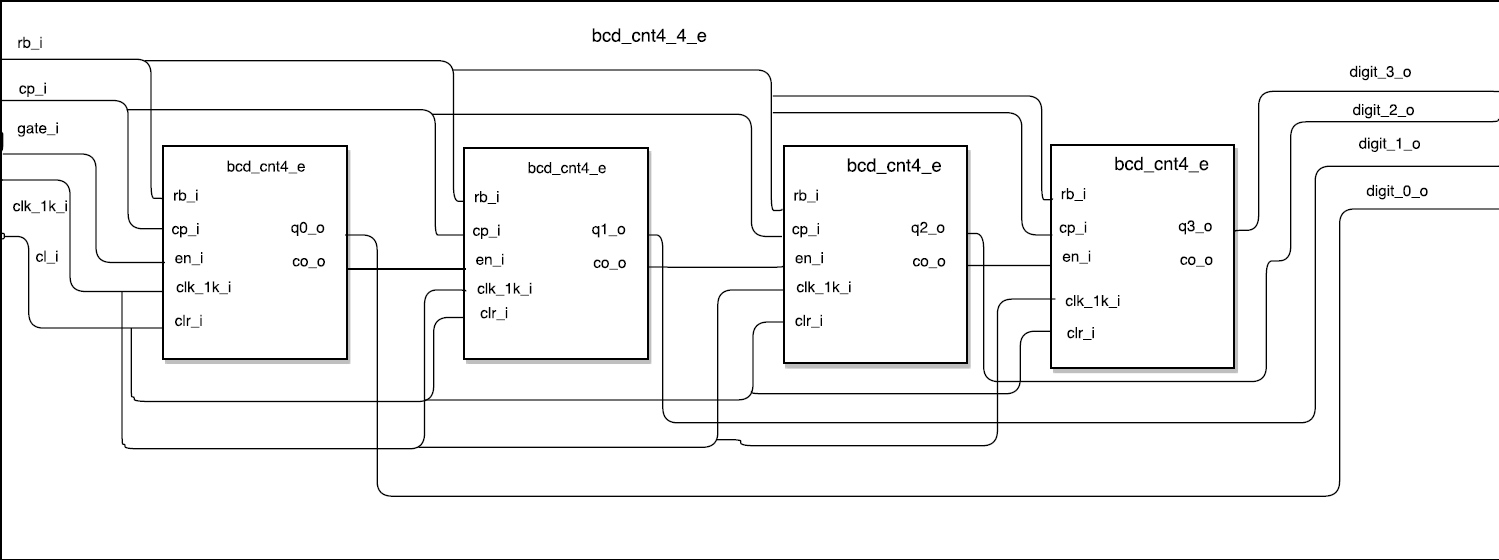
\includegraphics[width=16cm,height=8cm]{bcdcnt4arc.PNG}
\caption{architecture of the BCD counter}
\label{architecture of the BCD counter}
\end{figure}








The timing behaviour can be realised like :\\
\begin{figure}[H]
\centering
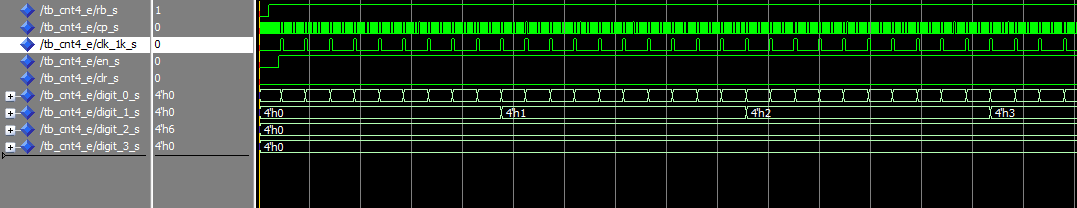
\includegraphics[width=16cm,height=6cm]{bcdcounter.PNG}
\caption{Timing behaviour of the BCD counter}
\label{Timing behaviour of the BCD counter}
\end{figure}

\subsection{BCD to ASCII conversion}
This is just a simple block that converts the value that has been counted by the BCD counter into the ASCII 8-bit vectors.\\ 

The entity seems to be like :\\
\begin{figure}[H]
\centering
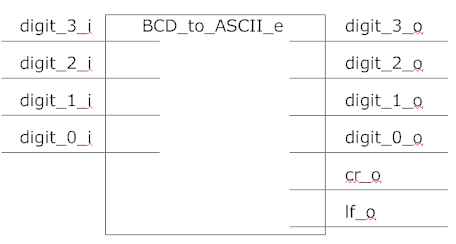
\includegraphics[width=8cm,height=6cm]{bcdAscii.PNG}
\caption{Entity of the BCD to ASCII }
\label{Entity of the BCD to ASCII }
\end{figure}

\subsection{Transmission (UART)}
As mentioned above, this block is responsible for transmitting the data that has been calculated by the FPGA chip to the computer. UART is a device that has the capabilities to both receive and transmit data. UART exchanges text data into American Standard Code For Information Interchange(ASCII)  format. In that, each alphabetical character is encoded by 7-bits and transmitted as 8 data bits. The transfer of the ASCII pattern is being done inside the transmission block(UART). For the transmission, the UART protocol wraps this 8-bit sub word with a start bit in the least significant bit and a stop bit in the most significant bit. The diagram shown below shows a lot of things about the UART:\\


\begin{figure}[H]
\centering
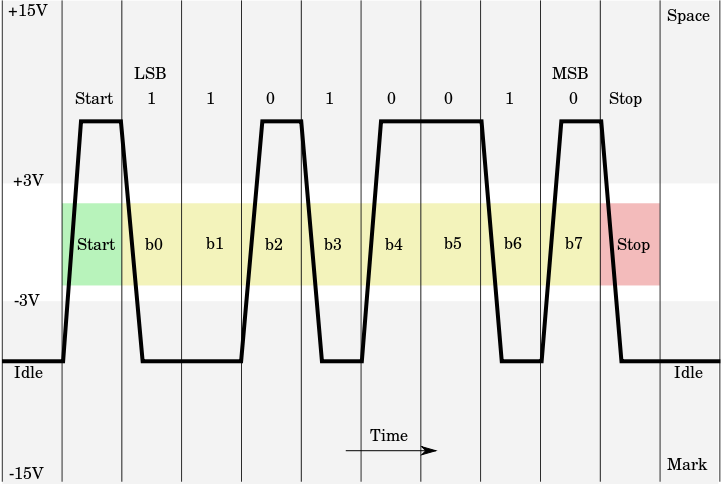
\includegraphics[width=16cm,height=6cm]{UARTprotocol.png}
\caption{UART protocol diagram}
\label{UART protocol diagram}
\end{figure}


UART transmitter controls transmission by fetching a data word in parallel format and directing the UART to transmit it in a serial format. Likewise, the Receiver must detect transmission, receive the data in serial format, strip of the start and stop bits, and store the data word in a parallel format. Since the UART is asynchronous in working, the receiver does not know when the data will come, so receiver generate local clock in order to synchronize to transmitter whenever start bit is received. Asynchronous transmission allows data to be transmitted without the sender having to send a clock signal to the receiver. The transmitter and receiver agree on timing parameters in advance and special bits are added to each word which is used to synchronize the sending and receiving units. When a word is given to the UART for Asynchronous transmission, a bit called the “Start Bit” is added to the beginning of each word that is to be transmitted. The Star Bit is used to alert the receiver that a word of data is about to be sent, and to force the clock in the receiver into synchronization with the clock in the transmitter. After the Start Bit, the individual bits of the word of data are sent, with the Least Significant Bit (LSB) being sent first. Each bit in the transmission is transmitted 
for exactly the same amount of time as all of the other bits, and the receiver “looks” at the wire at approximately halfway through the period assigned to each bit to determine if the bit is a $1$or a $0$. For example, if it takes two seconds to send each bit, the receiver will examine the signal to determine if it is a $1$ or a $0$ after one second has passed, then it will wait two seconds and then examine the value of the next bit, and so on. Then at least one $4$\ Stop Bit is sent by the transmitter. Because asynchronous data is “self-synchronous”, if there is no data to transmit, the transmission line can be idle.\\

This was the theory part. Let’s take a look at how this theory can be achieved. So far, the values from the BCD counter have been converted into the ASCII digits. In the transmission block, there are five blocks running side by side in order to transmit the data. \\


\begin{figure}[H]
\centering
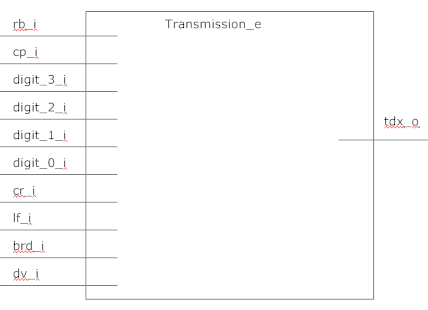
\includegraphics[width=8cm,height=6cm]{transmissionE.PNG}
\caption{Entity of the transmission block}
\label{Entity of the transmission block}
\end{figure}





\begin{figure}[H]
\centering
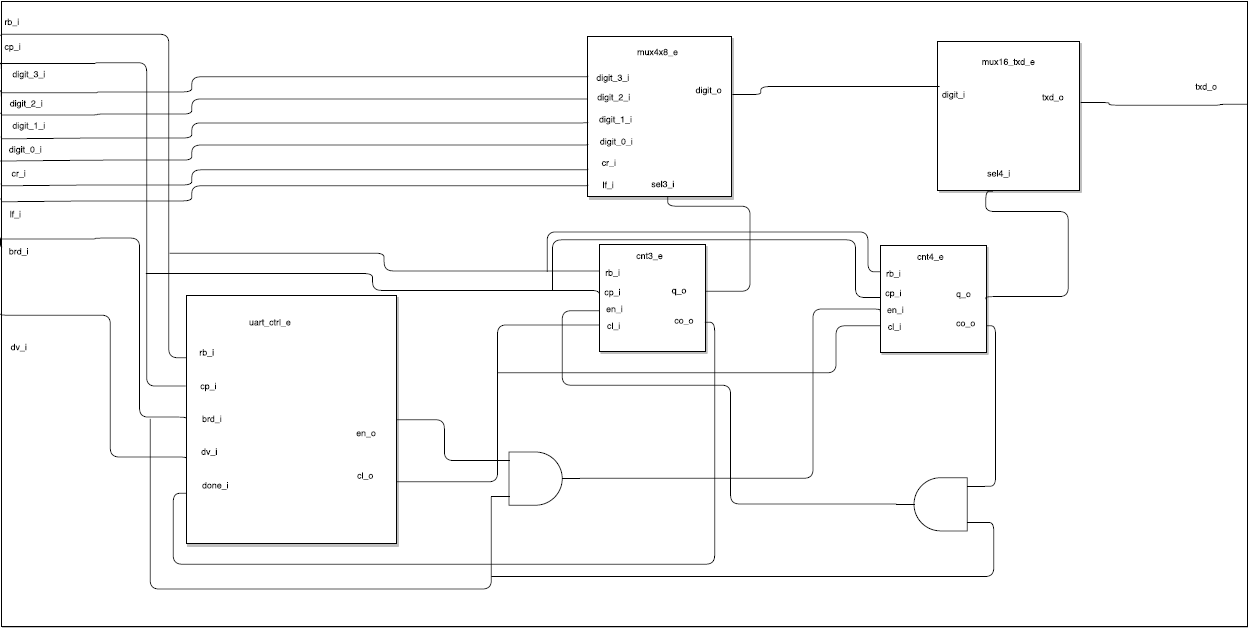
\includegraphics[width=16cm,height=8cm]{transmmistion.PNG}
\caption{Architecture of the transmission block}
\label{Architecture of the transmission block}
\end{figure}

In the diagram above, it can be see that there are two multiplexers that are selecting the transmittable data according to the selection bits from the two counters running behind it. The Multiplexer  mux4x8 selects the ASCII vector that needs to be transmitted. This selection is done by the selection bits, that are provided by the counter cnt3. The Multiplexer mux16\_txd is responsible for transmitting the data in the UART sequence corresponding to the selection bits that are provided by the counter cnt4.\\

The uart\_ctrl is the Finite State Machine that is being running behind the two counters and providing the data, when and which should be selecting simultaneously! The working of the FSM of uart\_ctrl can be easily understand by the state diagram. The way such state transition occurs is due to the requirement of feeding the data serially.\\

\begin{figure}[H]
\centering
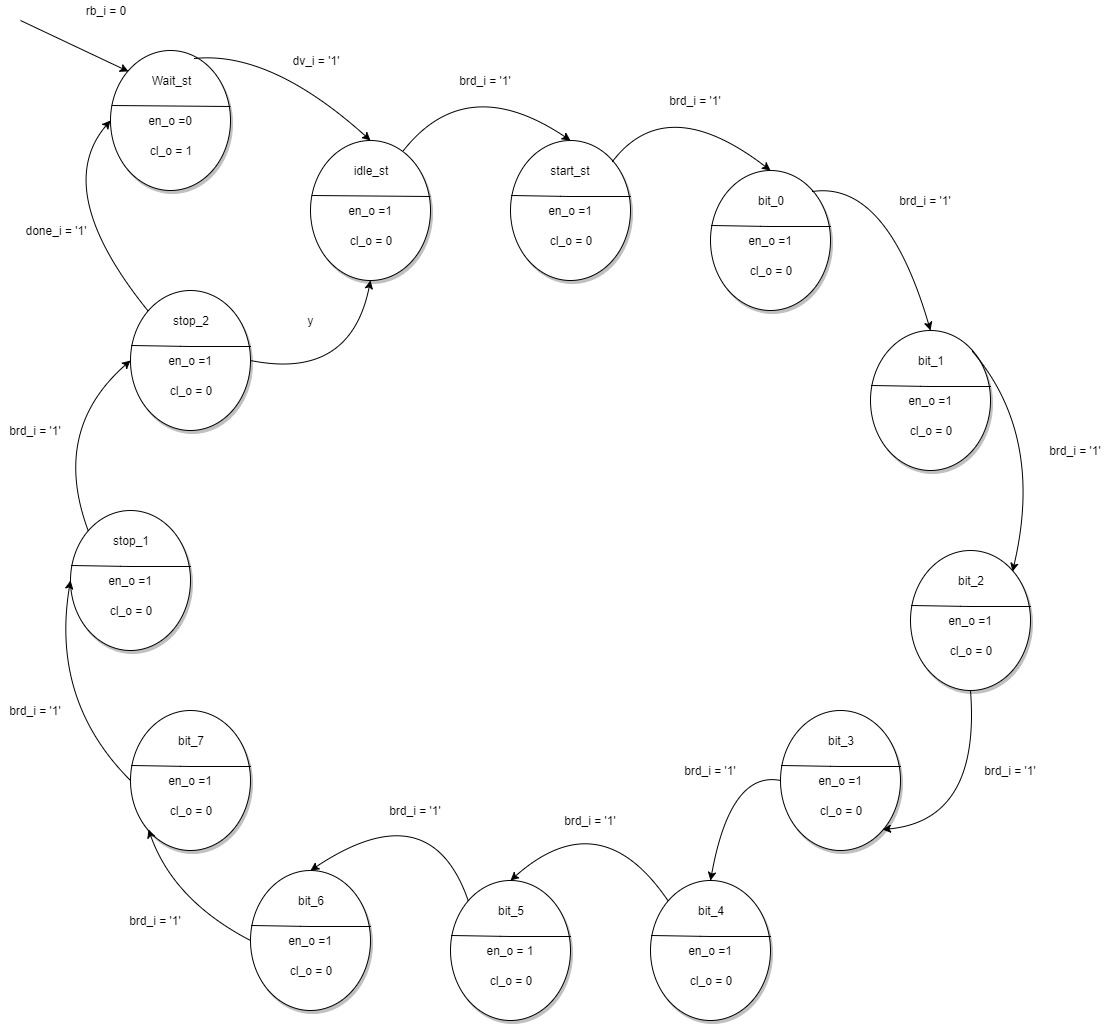
\includegraphics[width=10cm,height=11cm]{uartFsm.jpg}
\caption{UART FSM}
\label{UART FSM}
\end{figure}

The timing behaviour of the Transmission block looks like :\\

\begin{figure}[H]
\centering
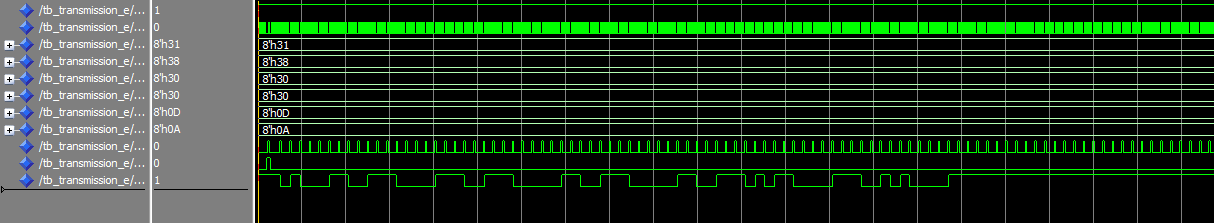
\includegraphics[width=16cm,height=5cm]{transmission.PNG}
\caption{The timing behavior of the transmission block}
\label{The timing behavior of the transmission block}
\end{figure}

\subsection{Output on PC}
The PC communicates with the whole system via UART communication. It communicates through the RS232DB9 COM port’s interface. It runs a C program reads the ASCII numbers from the COM port, converts them into integers, and display it on the Terminal. The figure of the C code is given below :\\

\begin{figure}[H]
\centering
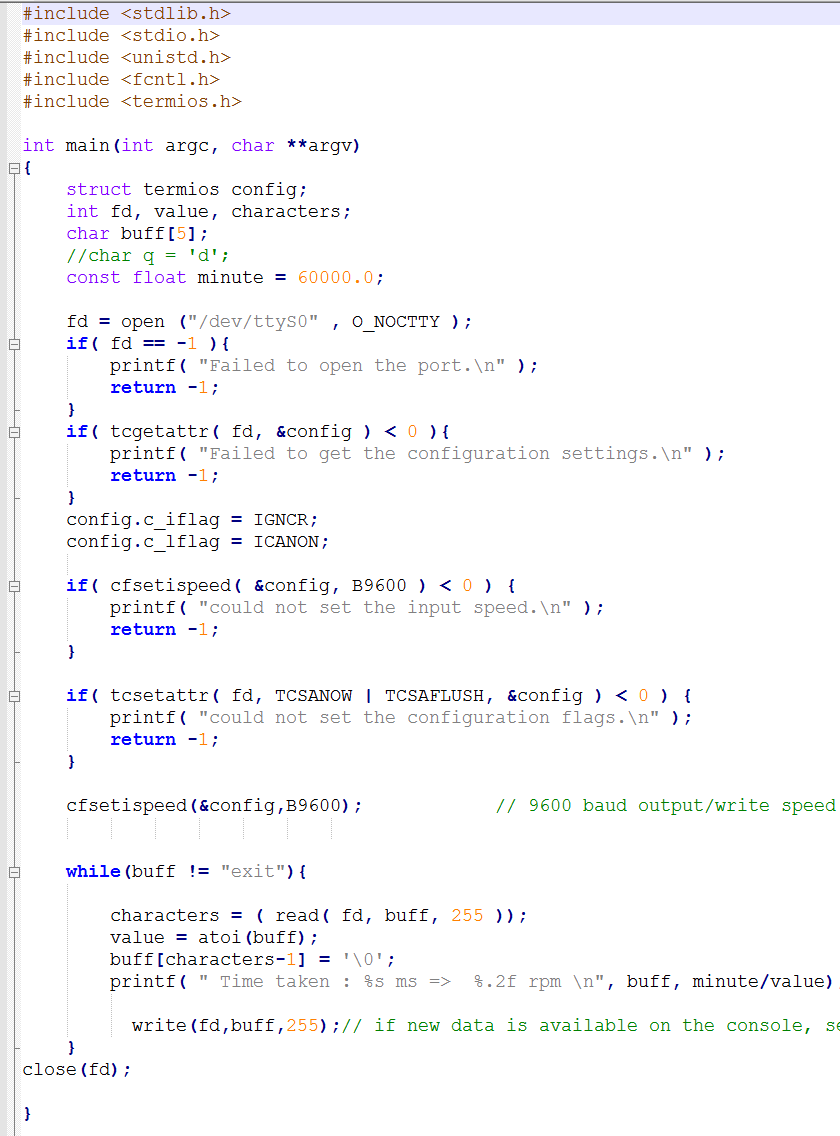
\includegraphics[width=\linewidth]{cprogram.PNG}
\caption{C program}
\label{C program}
\end{figure}

\subsection{System Active LED}
LED flashing at 1 Hz output:\\
\[ 
\frac{50 MHz}{1 Hz}= 50000000 clock cycles
\]
\subsection{Baud Rate Generator}
\[
 \frac{50 MHz}{9600 Hz}= 5208clock cycles
\]
\section{Test and Debug}
There has already been done a lot of testing with the proram and have got a bit similar results. The testing have been done using the Software ISE Design Suite and Simulation have been down using the Software Modelsim Simulator.\\
The values that has been printing on the Terminal, has been checked via GTKTerm. Then after, the C program has been used in order to print the result on the Terminal.\\
The testbench of the Top level architecture has been runned through and got some astonishing results. The Stimulation of the Testbench of the top level have been shown below.\\
\begin{figure}[H]
\centering
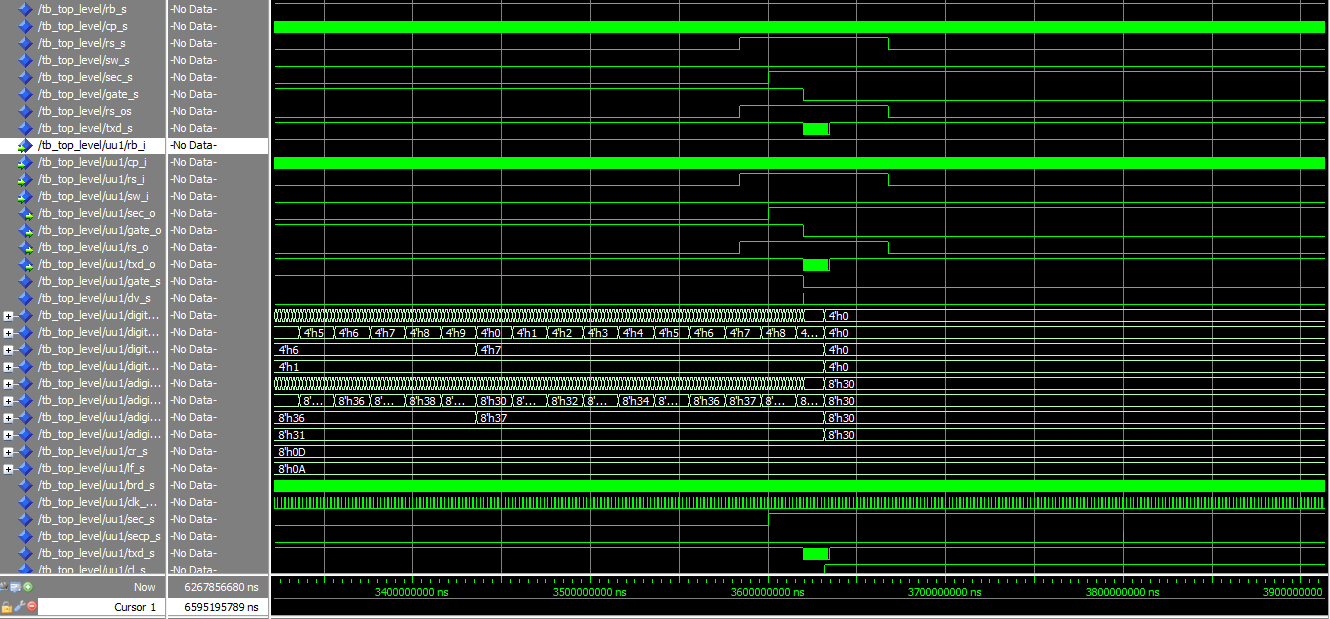
\includegraphics[width=16cm,height=10cm]{topleveltestbench.PNG}
\caption{Top level testbench stimulation}
\label{Top level testbench stimulation}
\end{figure}



The final result that has been achieved on gtkterm:\\
\begin{figure}[H]
\centering
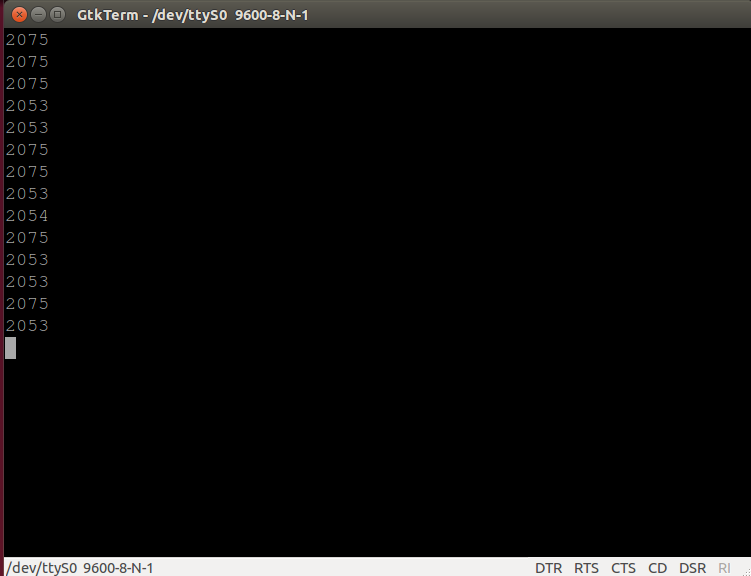
\includegraphics[width=16cm,height=9cm]{gtktermresult.png}
\caption{Final result on gtkterm}
\label{Final result}
\end{figure}







The final result that has been achieved :\\
\begin{figure}[H]
\centering
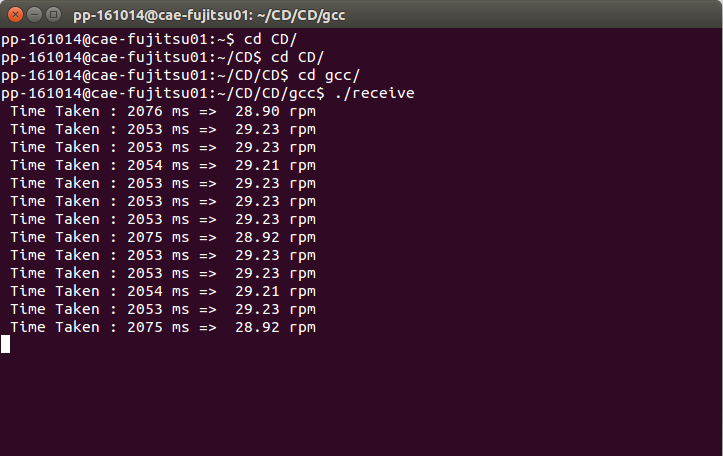
\includegraphics[width=16cm,height=9cm]{ccoderesult.png}
\caption{Final result}
\label{Final result}
\end{figure}



\newpage


\raggedright

\newpage                                                                                %biblography
%\section{Reference}
\begin{thebibliography}{}

\bibitem{Intro1}
\texttt{<https://en.wikipedia.org/wiki/Field-programmable\_gate\_array>}

\bibitem{Intro1}
\texttt{<https://www.xilinx.com/products/silicon-devices/fpga/what-is-an-fpga\newline .html>}


\bibitem{Intro3}
\texttt{<https://en.wikipedia.org/wiki/VHDL>}



\end{thebibliography}



\clearpage

\end{document}
